\section*{Reduction}
First, we define some variable for JSS problem. We have start ($S${\scriptsize$i,j$}) for the start time of $j$-th task for job $i$.  Each task start at $S${\scriptsize$i,j$} and run $T${\scriptsize$i,j$} units of time, where $T${\scriptsize$i,j$} denotes the duration of $j$-th task of job $i$. In classic JSS problem, there are only 2 constraints:

\begin{enumerate}
 \item Precedence \\
A precedence constraint between two consecutive tasks $T${\scriptsize$i,j$} and $T${\scriptsize$i,j+1$} is encoded using
the inequality $S${\scriptsize$i,j+1$} $\geq$ $S${\scriptsize$i,j$} + $S${\scriptsize$i,j$}. This inequality states that the start-time of task $j+1$ must be greater than or equal to the start-time of task $j$ plus its duration.


\item Resource Capacity \\
 A resource constraint between two tasks from different jobs $i$ and $i$' requiring the same machine $j$ is encoded using the formula \\
 ($S${\scriptsize$i,j$} $\geq$ $S${\scriptsize$i$',$j$} + $T${\scriptsize$i$',$j$}) $\vee$ ($S${\scriptsize$i$',$j$} $\geq$ $S${\scriptsize$i,j$} + $T${\scriptsize$i,j$}) , which states that the two tasks do not overlap. 


\end{enumerate}
Moreover, other than the 2 main constraints above, we need some other constraint in programming.

\begin{enumerate}
\setcounter{enumi}{2}
 \item  Start-time for the first task of each job need to be greater or equal to zero,
 that is\\ $S${\scriptsize$i$,0} $\geq$ 0



\item At the end, we define a variable $max$(makespan). And we want to decide if there is a schedule such that end-time of the last task is less or equal max time, that is $S${\scriptsize$i,n$} + $T${\scriptsize$i,n$} $\leq$ $max$(makespan), where $n$ is the index number of last task for each job.




\end{enumerate}
We conclude the constraints in arbitrary sentence in the following table. 

\begin{figure}[H]
\centering
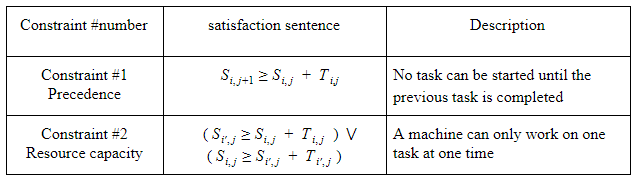
\includegraphics[width=6in]{img/2.PNG}

\end{figure}
We will continue using the example from Google project to generate the SMT formula:

\begin{figure}[H]
\centering
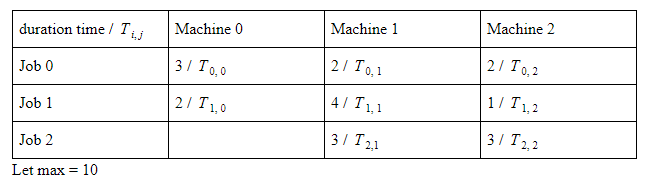
\includegraphics[width=6in]{img/3.PNG}

\end{figure}

\subsection*{Encoding:}
($S${\scriptsize0,0} $\geq$ 0) $\wedge$ ($S${\scriptsize0,1} $\geq$ $S${\scriptsize0,0} + 3) $\wedge$ ($S${\scriptsize0,2} $\geq$ $S${\scriptsize0,1} + 2) $\wedge$ ($S${\scriptsize0,2} + 2 $\leq$ 10) $\wedge$ \\
($S${\scriptsize1,0} $\geq$ 0) $\wedge$ ($S${\scriptsize1,1} $\geq$ $S${\scriptsize1,0} + 2) $\wedge$ ($S${\scriptsize1,2} $\geq$ $S${\scriptsize1,1} + 4) $\wedge$ ($S${\scriptsize1,2} + 1 $\leq$ 10) $\wedge$ \\
($S${\scriptsize2,1} $\geq$ 0) $\wedge$ ($S${\scriptsize2,2} $\geq$ $S${\scriptsize2,1} + 3)  $\wedge$ ($S${\scriptsize2,2} + 3 $\leq$ 10) $\wedge$ \\
(($S${\scriptsize0,0} $\geq$ $S${\scriptsize1,0} + 2) $\vee$ ($S${\scriptsize1,0} $\geq$ $S${\scriptsize0,0} + 3)) $\wedge$ \\
(($S${\scriptsize0,1} $\geq$ $S${\scriptsize1,1} + 4) $\vee$ ($S${\scriptsize1,1} $\geq$ $S${\scriptsize0,1} + 2)) $\wedge$ \\
(($S${\scriptsize0,1} $\geq$ $S${\scriptsize2,1} + 3) $\vee$ ($S${\scriptsize2,1} $\geq$ $S${\scriptsize0,1} + 2)) $\wedge$ \\
(($S${\scriptsize1,1} $\geq$ $S${\scriptsize2,1} + 3) $\vee$ ($S${\scriptsize2,1} $\geq$ $S${\scriptsize1,1} + 4)) $\wedge$ \\
(($S${\scriptsize0,2} $\geq$ $S${\scriptsize1,2} + 1) $\vee$ ($S${\scriptsize1,2} $\geq$ $S${\scriptsize0,2} + 2)) $\wedge$ \\
(($S${\scriptsize0,2} $\geq$ $S${\scriptsize2,2} + 3) $\vee$ ($S${\scriptsize2,2} $\geq$ $S${\scriptsize0,2} + 2)) $\wedge$ \\
(($S${\scriptsize1,2} $\geq$ $S${\scriptsize2,2} + 3) $\vee$ ($S${\scriptsize2,2} $\geq$ $S${\scriptsize1,2} + 1)) 